%%%%%%%%%%%%%%%%%%%%%%%%%%%%%%%%%%%%%%%%%%%%%%%%%%%%%%%%%%%%%%%%%%%%%%%%
% Uni Duesseldorf
% Lehrstuhl fuer Datenbanken und Informationssysteme
% Vorlage fuer Bachelor-/Masterarbeiten
% Optimiert fuer den Original-Latex-Kompiler LATEX.EXE (LaTeX=>PS=>PDF)
%%%%%%%%%%%%%%%%%%%%%%%%%%%%%%%%%%%%%%%%%%%%%%%%%%%%%%%%%%%%%%%%%%%%%%%%
% Ueberarbeitung für pdflatex (LaTeX=>PDF)
%%%%%%%%%%%%%%%%%%%%%%%%%%%%%%%%%%%%%%%%%%%%%%%%%%%%%%%%%%%%%%%%%%%%%%%%
% Vorlage Changelog:
% 10.09.2015 (Matthias Liebeck): Nummerierung des Inhaltsverzeichnis nun römisch, Beispiel für einen Anhang eingebaut, \raggedbottom hinter sections eingefügt
% 11.07.2018 (Matthias Liebeck): Ersetzung des Bibliographiestils, Einsatz von Biber
% 04.09.2018 (Matthias Liebeck):
%   * Bibtex: unnötige Bibtexfelder beim Rendern ausblenden (thx @ Markus Brenneis)
%   * ngerman: "et al." im BibTeX für drei oder mehr Autoren
%   * Neuer Befehl \sectionforcestartright: Sections immer rechts beginnen (thx @ Philipp Grawe)
%   * ngerman: Deutsche Anführungszeichen im Literaturverzeichnis (thx @ Markus Brenneis)
%   * ngerman: Deutsche Anführungszeichen im Literaturverzeichnis (thx @ Markus Brenneis)
% 16.10.2018 (Matthias Liebeck): Zwei fixes an \sectionforcestartright (thx @ Markus Brenneis)
%%%%%%%%%%%%%%%%%%%%%%%%%%%%%%%%%%%%%%%%%%%%%%%%%%%%%%%%%%%%%%%%%%%%%%%%
%%%% BEGINN EINSTELLUNG FUER DIE ARBEIT. UNBEDINGT ERFORDERLICH! %%%%%%%
%%%%%%%%%%%%%%%%%%%%%%%%%%%%%%%%%%%%%%%%%%%%%%%%%%%%%%%%%%%%%%%%%%%%%%%%
% Geben Sie Ihren Namen hier an:

\newcommand{\bearbeiter}{Robin Kösters}

% Geben Sie hier den Titel Ihrer Arbeit an:
\newcommand{\titel}{Klassifikation von Tweets zur Erkennung von Trollen}

% Geben Sie das Datum des Beginns und Ende der Bachelorarbeit ein:
\newcommand{\beginndatum}{18. September 2020}
\newcommand{\abgabedatum}{18.~Dezember~2020}

% Geben Sie die Namen des Erst- und Zweitgutachters an:
\newcommand{\erstgutachter}{Prof. Dr.~Stefan Conrad}
\newcommand{\zweitgutachter}{Prof. Dr.~Martin Mauve}

% Falls Sie die Arbeit zweiseitig ausdrucken wollen,
% benutzen Sie die folgende Zeile mit
% \AN fuer zweiseitigen Druck
% \AUS fuer einseitigen Druck
\newcommand{\zweiseitig}{\AN}
% true fuer biber, false fuer klassischen Zitierstil
%\newcommand{\biber}{false}
\newcommand{\biber}{true}

% Falls Sections immer rechts beginnen sollen. Gerade für Masterarbeiten
% interessant. Bei kurzen Bachelorarbeiten eher weniger zu verwenden.
\newcommand{\sectionforcestartright}{false}
%\newcommand{\sectionforcestartright}{true}

% Falls die Arbeit in englischer Sprache verfasst
% werden soll, dann benutzen Sie die folgende Zeile mit
% englisch fuer englische Sprache
% deutsch fuer deutsche Sprache
\newcommand{\sprache}{deutsch}

% Hier wird eingestellt, ob es sich bei der Arbeit um eine Bachelor-
% oder Masterarbeit handelt (unpassendes auskommentieren!):
\newcommand{\arbeit}{Bachelorarbeit}
%~ \newcommand{\arbeit}{Masterarbeit}


%%%%%%%%%%%%%%%%%%%%%%%%%%%%%%%%%%%%%%%%%%%%%%%%%%%%%%%%%%%%%%%%%%%%%%%%
%%%% ENDE EINSTELLUNGEN %%%%%%%%%%%%%%%%%%%%%%%%%%%%%%%%%%%%%%%%%%%%%%%%
%%%%%%%%%%%%%%%%%%%%%%%%%%%%%%%%%%%%%%%%%%%%%%%%%%%%%%%%%%%%%%%%%%%%%%%%

% Die folgende Zeile NICHT EDITIEREN oder loeschen


%%%%%%%%%%%%%%%%%%%%%%%%%%%%%%%%%%%%%%%%%%%%%%%%%%%%%%%%%%%
% Obere Titelmakros. Editieren Sie diese Datei nur, wenn
% Sie sich ABSOLUT sicher sind, was Sie da tun!!!
% (Z.B. zum Abaendern der BA-Vorlage in eine MA-Vorlage)
% Uni Duesseldorf
% Lehrstuhl fuer Datenbanken und Informationssysteme
% Version 2.2 - 2.3.2010
%%%%%%%%%%%%%%%%%%%%%%%%%%%%%%%%%%%%%%%%%%%%%%%%%%%%%%%%%%%
\newcommand{\AN}{twoside}
\newcommand{\AUS}{}


%\newcommand{\englisch}{}
%\newcommand{\deutsch}{\usepackage[german]{babel}}

%% Die folgenden auskommentierten Optionen dienen der automatischen
%% Erkennung des Latex-Kompilers und dem Setzen der davon abhängigen
%% Einstellungen. Bei Problem z.B. mit dem Einbinden von verschiedenen
%% Grafiktypen bei Verwendung von PdfLatex oder Latex, einfach die
%% verschiedenen \usepackage(s) ausprobieren. (Mit diesen Einstellungen
%% funktionierte diese Vorlage bei der Verwenundg von latex.exe als
%% Kompiler bei den meisten Studierenden.)

%\newif\ifpdf \ifx\pdfoutput\undefined
%\pdffalse % we are not running pdflatex
%\else
%\pdfoutput=1 % we are running pdflatex
%\pdfcompresslevel=9 % compression level for text and image;
%\pdftrue \fi

\documentclass[11pt,a4paper, \zweiseitig]{article}
\usepackage{ifthen}


%\usepackage[iso]{umlaute}
\usepackage[utf8]{inputenc}
\usepackage{palatino} % palatino Schriftart
%\usepackage{makeidx} % um ein Index zu erstellen
\usepackage[nottoc]{tocbibind}
\usepackage[T1]{fontenc} %fuer richtige Trennung bei Umlauten
\usepackage{fancybox} % fuer die Rahmen
\usepackage{shortvrb}
\usepackage{url}
\usepackage{xcolor}
\usepackage[colorlinks,citecolor=blue,linkcolor=black]{hyperref} %anklickbares Inhaltsverzeichnis

\ifthenelse{\boolean{\biber}}{
  % only needed for biber
  \usepackage[style=authoryear,natbib=true,backend=biber,mincitenames=1,maxcitenames=2,maxbibnames=99,uniquelist=false,dashed=false]{biblatex}

  % https://tex.stackexchange.com/a/334703/8850
  \AtEveryBibitem{%
    \clearfield{issn}
    \clearfield{isbn}
    \clearfield{doi}
    \clearfield{location}
    \clearlist{location}
    \clearlist{address}

    \ifentrytype{online}{}{% Remove url except for @online
      \clearfield{url}
    }
  }
}
{}%no else

% Falls es bei \citet ein Komma zwischen Name und Jahr gibt:
% https://tex.stackexchange.com/questions/312539/unwanted-comma-between-author-and-year-using-citet-command
% (thx @ Markus Brenneis)
%\DeclareDelimFormat[cbx@textcite]{nameyeardelim}{\addspace}



\ifthenelse{\equal{\sprache}{deutsch}}{
  \usepackage[ngerman]{babel}
  % Bibtex u.a -> et al.
  \ifthenelse{\boolean{\biber}}{
    \DefineBibliographyStrings{ngerman}{
      andothers = {{et\,al\adddot}},
    }
    \newcommand{\references}{Literatur}
  }
  {} % do nothing when not using biber
  \usepackage[autostyle, german=quotes]{csquotes} % Deutsche Anführungszeichen im Literaturverzeichnis (thx @ Markus Brenneis)

}{ \newcommand{\references}{References}}

\usepackage{a4wide} % ganze A4 Weite verwenden



%\ifpdf
%\usepackage[pdftex,xdvi]{graphicx}
%\usepackage{thumbpdf} %thumbs fuer Pdf
%\usepackage[pdfstartview=FitV]{hyperref} %anklickbares Inhaltsverzeichnis
%\else
%\usepackage[dvips,xdvi]{graphicx}
\usepackage{graphicx}

%\fi

\newcommand{\redt}[1] {
  \textcolor{red}{#1}}

\newcommand{\oranget}[1] {
  \textcolor{orange}{#1}}

\newcommand{\purplet}[1] {
  \textcolor{purple}{#1}}

%%%%%%%%%%%%%%%%%%%%%%% Massangaben fuer die Arbeit %%%%%%%%%%%%%%%
\setlength{\textwidth}{15cm}

\setlength{\oddsidemargin}{35mm}
\setlength{\evensidemargin}{25mm}

\addtolength{\oddsidemargin}{-1in}
\addtolength{\evensidemargin}{-1in}

\ifthenelse{\boolean{\biber}}{\addbibresource{references.bib}}{}

%\makeindex
\begin{document}
%\setcounter{secnumdepth}{4} %Nummerieren bis in die 4. Ebene
%\setcounter{tocdepth}{4} %Inhaltsverzeichnis bis zur 4. Ebene

\pagestyle{headings}

\sloppy % LaTeX ist dann nicht so streng mit der Silbentrennung
%~ \MakeShortVerb{\§}

\parindent0mm
\parskip0.5em


{
\textwidth170mm
\oddsidemargin30mm
\evensidemargin30mm
\addtolength{\oddsidemargin}{-1in}
\addtolength{\evensidemargin}{-1in}

\parskip0pt plus2pt

% Die Raender muessen eventuell fuer jeden Drucker individuell eingestellt
% werden. Dazu sind die Werte fuer die Abstaende `\oben' und `\links' zu
% aendern, die von mir auf jeweils 0mm eingestellt wurden.

%\newlength{\links} \setlength{\links}{10mm}  % hier abzuaendern
%\addtolength{\oddsidemargin}{\links}
%\addtolength{\evensidemargin}{\links}

\begin{titlepage}
\vspace*{-1.5cm}
\raisebox{17mm}{
    \begin{minipage}[t]{70mm}
        \begin{center}
            %\selectlanguage{german}
            {\Large INSTITUT FÜR INFORMATIK\\}
            {\normalsize
                Datenbanken und Informationssysteme\\
            }
            \vspace{3mm}
            {\small Universitätsstr. 1 \hspace{5ex} D--40225 Düsseldorf\\}
        \end{center}
    \end{minipage}
}
\hfill
\raisebox{7mm}{
    
\includegraphics[width=130pt]{bilder/HHU_Logo}}
\vspace{14em}

% Titel
\begin{center}
    \baselineskip=55pt
    \textbf{\huge \titel}
    \baselineskip=0 pt
\end{center}

%\vspace{7em}

\vfill

% Autor
\begin{center}
    \textbf{\Large
        \bearbeiter
    }
\end{center}

\vspace{35mm}

% Prüfungsordnungs-Angaben
\begin{center}
%\selectlanguage{german}

%%%%%%%%%%%%%%%%%%%%%%%%%%%%%%%%%%%%%%%%%%%%%%%%%%%%%%%%%%%%%%%%%%%%%%%%%
% Ja, richtig, hier kann die BA-Vorlage zur MA-Vorlage gemacht werden...
% (nicht mehr nötig!)
%%%%%%%%%%%%%%%%%%%%%%%%%%%%%%%%%%%%%%%%%%%%%%%%%%%%%%%%%%%%%%%%%%%%%%%%%
{\Large \arbeit}

\vspace{2em}
\ifthenelse{\equal{\sprache}{deutsch}}{
    \begin{tabular}[t]{ll}
    Beginn der Arbeit:& \beginndatum \\
    Abgabe der Arbeit:& \abgabedatum \\
    Gutachter:         & \erstgutachter \\
    & \zweitgutachter \\
}{
    \begin{tabular}[t]{ll}
    Date of issue:& \beginndatum \\
    Date of submission:& \abgabedatum \\
    Reviewers:         & \erstgutachter \\
    & \zweitgutachter \\
}
\end{tabular}
\end{center}

\end{titlepage}

}

%%%%%%%%%%%%%%%%%%%%%%%%%%%%%%%%%%%%%%%%%%%%%%%%%%%%%%%%%%%%%%%%%%%%%
\clearpage
\begin{titlepage}
    ~                % eine leere Seite hinter dem Deckblatt
\end{titlepage}
%%%%%%%%%%%%%%%%%%%%%%%%%%%%%%%%%%%%%%%%%%%%%%%%%%%%%%%%%%%%%%%%%%%%%
\clearpage
\begin{titlepage}
    \vspace*{\fill}

    \section*{Erklärung}

    %%%%%%%%%%%%%%%%%%%%%%%%%%%%%%%%%%%%%%%%%%%%%%%%%%%%%%%%%%%
    % Und hier ebenfalls ggf. BA durch MA ersetzen...
    % (Auch nicht mehr nötig!)
    %%%%%%%%%%%%%%%%%%%%%%%%%%%%%%%%%%%%%%%%%%%%%%%%%%%%%%%%%%%

    Hiermit versichere ich, dass ich diese \arbeit{}
    selbstständig verfasst habe. Ich habe dazu keine anderen als die
    angegebenen Quellen und Hilfsmittel verwendet.

    \vspace{25 mm}

    \begin{tabular}{lc}
        Düsseldorf, den \abgabedatum \hspace*{2cm} & \underline{\hspace{6cm}} \\
                                                   & \bearbeiter
    \end{tabular}

    \vspace*{\fill}
\end{titlepage}

%%%%%%%%%%%%%%%%%%%%%%%%%%%%%%%%%%%%%%%%%%%%%%%%%%%%%%%%%%%%%%%%%%%%%
% Leerseite bei zweiseitigem Druck
%%%%%%%%%%%%%%%%%%%%%%%%%%%%%%%%%%%%%%%%%%%%%%%%%%%%%%%%%%%%%%%%%%%%%

\ifthenelse{\equal{\zweiseitig}{twoside}}{\clearpage\begin{titlepage}
        ~\end{titlepage}}{}

%%%%%%%%%%%%%%%%%%%%%%%%%%%%%%%%%%%%%%%%%%%%%%%%%%%%%%%%%%%%%%%%%%%%%
\clearpage
\begin{titlepage}

    %%% Die folgende Zeile nicht ändern!
\section*{\ifthenelse{\equal{\sprache}{deutsch}}{Zusammenfassung}{Abstract}}
%%% Zusammenfassung:
Hier kommt eine ca.\ einseitige Zusammenfassung der Arbeit rein.



    %%%%%%%%%%%%%%%%%%%%%%%%%%%%%%%%%%%%%%%%%%%%%%%%
    % Untere Titelmakros. Editieren Sie diese Datei nur, wenn Sie sich
    % ABSOLUT sicher sind, was Sie da tun!!!
    %%%%%%%%%%%%%%%%%%%%%%%%%%%%%%%%%%%%%%%%%%%%%%%
    \vspace*{\fill}
\end{titlepage}

%%%%%%%%%%%%%%%%%%%%%%%%%%%%%%%%%%%%%%%%%%%%%%%%%%%%%%%%%%%%%%%%%%%%%
% Leerseite bei zweiseitigem Druck
%%%%%%%%%%%%%%%%%%%%%%%%%%%%%%%%%%%%%%%%%%%%%%%%%%%%%%%%%%%%%%%%%%%%%
\ifthenelse{\equal{\zweiseitig}{twoside}}
{\clearpage\begin{titlepage}~\end{titlepage}}{}
%%%%%%%%%%%%%%%%%%%%%%%%%%%%%%%%%%%%%%%%%%%%%%%%%%%%%%%%%%%%%%%%%%%%%
\clearpage \setcounter{page}{1}
\pagenumbering{roman}
\setcounter{tocdepth}{2}
\tableofcontents

%\enlargethispage{\baselineskip}
\clearpage
%%%%%%%%%%%%%%%%%%%%%%%%%%%%%%%%%%%%%%%%%%%%%%%%%%%%%%%%%%%%%%%%%%%%%
% Leere Seite, falls Inhaltsverzeichnis mit ungerader Seitenzahl und
% doppelseitiger Druck
%%%%%%%%%%%%%%%%%%%%%%%%%%%%%%%%%%%%%%%%%%%%%%%%%%%%%%%%%%%%%%%%%%%%%
\ifthenelse{ \( \equal{\zweiseitig}{twoside} \and \not \isodd{\value{page}} \)}
{\pagebreak \thispagestyle{empty} \cleardoublepage}{\clearpage}


% Kapitel soll bei doppelseitigem Druck immer auf der rechten (ungeraden) Seite anfangen (thx @ Philipp Grawe)
% https://tex.stackexchange.com/a/223387
\ifthenelse{\boolean{\sectionforcestartright}}
{\let\oldsection\section % Store \section in \oldsection
    \renewcommand{\section}{\cleardoublepage\oldsection}}
{}
\pagenumbering{arabic}
\setcounter{page}{1}

%%%%%%%%%%%%%%%%%%%%%%%%%%%%%%%%%%%%%%%%%%%%%%%%%%%%%%%%%%%%%%%%%%%%%%%%
%%%% BEGINN TEXTTEIL %%%%%%%%%%%%%%%%%%%%%%%%%%%%%%%%%%%%%%%%%%%%%%%%%%%
%%%%%%%%%%%%%%%%%%%%%%%%%%%%%%%%%%%%%%%%%%%%%%%%%%%%%%%%%%%%%%%%%%%%%%%%

%%%%%%%%%%%%%%%%%%%%%%%%%%%%%%%%%%%%%%%%%%%%%%%%%%%%%%%%%%%%%%%%%%%%%%%%
% Text entweder direkt hier hinein schreiben oder, im Sinne der
% besseren Uebersichtlich- und Bearbeitbarkeit mittels \input die
% einzelnen Textteile hier einbinden.
%%%%%%%%%%%%%%%%%%%%%%%%%%%%%%%%%%%%%%%%%%%%%%%%%%%%%%%%%%%%%%%%%%%%%%%%

\section{Einleitung}\raggedbottom
\subsection{Motivation}
Die US-Präsidentschaftswahl 2016 gilt vielen politischen Beobachtern als eindrucksvollstes Beispiel dafür, wie von staatlicher Seite organisierte Desinformationskampagnen den politischen Diskurs nachhaltig verzerren können. Bereits zwei Jahre nach der Wahl kamen britische Wissenschaftler in Zusammenarbeit mit der Firma Graphika zu der Erkenntnis, dass ein Unternehmen mit dem Namen \glqq Internet Research Agency\grqq{}	(IRA), welches dem russischen Staat nahesteht, im großen Stil versucht hat, amerikanische Wähler via Fake-Postings in sozialen Netzwerken zu beeinflussen. In ihrem Bericht geben die Forscher an, dass mehr als 30 Millionen Benutzer im Zeitraum von 2015 bis 2017 in Berührung mit von der IRA erstellten Inhalten gekommen sind. Die Urheber jener destruktiver Inhalte werden Trolle genannt. \citep{IRAOxf18}\\
In Twitter, welches das hauptsächlich betrachtete soziale Netzwerk in dieser Arbeit sein soll, machen Trolle besonders von der Hashtag-Setzung Gebrauch. Bei einem \textit{Hashtag} handelt es sich um eine durch den Ersteller eines Beitrags vorgenommene Themenfestlegung bzw. -klassifizierung. Eine nicht durch Leerzeichen unterbrochene Zeichenkette wird durch Voranstellen eines Rautezeichens (engl. \textit{hash}) zu einem Hashtag. In der Folge kann ein \textit{Tweet} (plattformeigene Bezeichnung für einen Beitrag) durch das Benutzen der allgemeinen Suchfunktion gefunden werden. Abbildung \ref{tweetex} zeigt einen beispielhaften Tweet der IRA, welcher dem der Arbeit zugrundeliegenden Datensatz entnommen wurde und die Hashtag-Nutzung durch einen Troll illustriert.
\begin{figure}[htb]
	\begin{center}
		
\includegraphics{bilder/Abb1.png}
		\caption{Beispiel eines IRA-Tweets}\label{tweetex}
	\end{center}
\end{figure}\\
Kommt es innerhalb eines gewissen Zeitraums zur gehäuften Benutzung eines bestimmten Hashtags, so wird dieser in den \glqq Twitter-Trends\grqq, eine Art Ranking der momentan meistgenutzten Hashtags, aufgeführt. Dies macht die Aktualität bzw. Relevanz eines gesellschaftlichen Themas direkt ablesbar. Für Trolle bietet dies aber die Möglichkeit durch geschickte zeitliche Abstimmung bestimmte Hashtags zu Trend-Hashtags zu machen und den Nutzern so aktiv die Relevanz bestimmter Themen vorzutäuschen.\\
Insgesamt sind mit den genannten Methoden verschiedenste Arten der Manipulation seitens Trollen denkbar. So können Trolle eine politische Partei oder einen Kandidaten unterstützen und versuchen, ihren Mitbewerbern zu schaden. Beispiele dafür gibt es auch in Deutschland.
So gelang es dem ultrarechten Netzwerk \glqq Reconquista Germanica\grqq{} während des TV-Duells zwischen Bundeskanzlerin Merkel und ihrem Herausforderer Martin Schulz im Jahr 2017 reichweitenstarke Tweets zu erstellen, welche Politiker diskreditieren \citep{tagesschau2020}.
Ein weitere tragende Säule von Desinformationskampagnen, welche meist in Verbindung zu Trollen steht, sind die \textit{Fake News}. Hierbei handelt es sich um Falschmeldungen bzw. Nachrichten ohne Wahrheitsgehalt, welche verbreitet werden, um die Öffentlichkeit zu manipulieren. Trolle treten hier in der Regel wechselweise als Urheber und Multiplikatoren solcher Meldungen auf.\\
Alle bisher beschriebenen Strategien sind gemeinsam als integrative Gesamtstrategie dazu geeignet, um die Ausgänge demokratischer Wahlen zu beeinflussen. Die Initiative \glqq ichbinhier e.V.\grqq{} und das Londoner \glqq Institute for Strategic Dialogue\grqq{} (ISD) kamen in einer Studie beispielsweise zu der Schlüsselerkenntnis, dass rechtsextreme Trollnetzwerke im Bundestagswahlkampf 2017 Urheber einer ausgedehnten und erfolgreichen \glqq pro-AfD-Wahlkampagne\grqq{} waren \citep{ISD18}. Das Ziel der Desinformationskampagnen, gleich ob aus dem Inland oder Ausland gesteuert, ist die Destabilisierung der demokratischen Institutionen bzw. der Demokratie als Ganzes. Aus diesem Grund möchte ich in meiner Abschlussarbeit einen Teil dazu beitragen, dass eine Lösung für dieses Problem gefunden wird.  
\subsection{Datensätze}
Im Rahmen dieser Arbeit sollen Verfahren beschrieben werden, welche die zuverlässige Erkennung von Troll-Inhalten auf Twitter ermöglichen. Hierbei kommen verschiedenste Techniken der Textklassifikation zum Einsatz, welche vorliegende Tweets entweder den Troll-Tweets oder den Nichttroll-Tweets zuordnen sollen. Sie werden auf zwei Datensätze angewandt, auf deren Eigenschaften und Ursprünge an dieser Stelle eingegangen werden soll.\\
Die Grundmenge des ersten Datensatzes ist eine von \citet{LinWar18} veröffentlichte Sammlung von rund 3 Millionen Tweets der IRA. Hier wurden die Tweets mit den zehn häufigsten Hashtags entnommen.\\
Beim zweiten Datensatz handelt es sich um im Vorfeld eigens extrahierte Tweets von echten Profilen. Um eine thematische Ähnlichkeit herzustellen, wurden nur Tweets mit den gleichen Hashtags wie im ersten Datensatz ausgewählt. Dies ist entscheidend, da eine thematische Ferne gleichbedeutend mit einer zu offensichtlichen Unterscheidbarkeit ist. Die Ergebnisse der Klassifikation wären in diesem Fall erwartbar klar und würden damit einen geminderten praktischen Nutzen nach sich ziehen. Es ist in diesem Zusammenhang auch nicht unwichtig, dass Trolle sich oftmals als authentische Benutzer tarnen und in deren Diskussionsräume vordringen. Die Ergebnisse sind erst dann von Wert, wenn auch diese, in der Theorie schwieriger zu unterscheidenden User, gut unterschieden werden. Aus jenen genannten Gründen ist die thematische Nähe beider Datensätze von entscheidender Bedeutung. Weiterhin wurde darauf geachtet, dass die Hashtags ungefähr gleich unter den Tweets verteilt sind. Tabelle \ref{dist_hashtags} zeigt den prozentualen Anteil eines jeden Hashtags am Gesamtdatensatz. Hier sind Differenzen von höchstens 5\%, meist aber um die 1\% zu beobachten.\\
\begin{table}[htb]
	\begin{center}
		\begin{tabular}{|l|l|l||l|l|l|}
			\hline
			Hashtag & Troll & Nichttroll & Hashtag & Troll & Nichttroll  \\ \hline \hline
			\#news	   & 42,50\%  & 40,50\% & \#topNews           & 05,00\% & 05,87\% \\ \hline
			\#sports   & 16,06\%  & 15,99\% &  \#MAGA             & 05,07\% & 05,23\% \\
			\#politics & 13,12\%  & 15,25\% & \#BlackLivesMatter  & 03,96\% & 04,56\% \\
			\#world	   & 09,13\%   & 13,94\% & \#health            & 03,84\% & 04,60\% \\
			\#local	   & 08,62\%   & 08,83\%  & \#tcot               & 03,99\% & 05,93\% \\ \hline			
		\end{tabular}
		\caption{Verteilung der Hashtags}\label{dist_hashtags}
	\end{center}
\end{table}\\
Zur Sicherheit wurde am Ende der Extraktion die Mengendifferenz beider Datensätze gebildet um die Datensätze streng disjunkt zu halten.\\
Der neu entstehende zusammengesetzte Datensatz besteht aus knapp 630.000 Tweets. 
Tabelle \ref{tab_datasets} zeigt zum Vergleich die wichtige Kennzahlen beider Bestandteile wie den Erstellungszeitraum und die durchschnittliche Länge der Zeichenketten.
\begin{table}[htb]
	\begin{center}
		\begin{tabular}{|l|l|l|}
			\hline
		Eigenschaft					& Troll		& Nichttroll\\ \hline \hline
		Anzahl Tweets   			& 303.036	& 324.873	\\ \hline
		unterschiedliche Autoren    & 770		& 68.706		\\ \hline
		Zeitraum					& 01/2015 - 09/2017& 01/2015 - 05/2018\\ \hline
		durchschnittliche Länge		& 78,64 Zeichen	& 122,27 Zeichen\\ \hline
		\end{tabular}
		\caption{Vergleich der Datensätze}\label{tab_datasets}
	\end{center}
\end{table}
\pagebreak
\section{Grundlagen des Text Mining}\raggedbottom
Im nachfolgenden Kapitel werden jene Konzepte des \textit{Text Minings} erläutert, welche grundlegend für das Verständnis von Methoden der Textklassifikation sind. Abbildung \ref{pipetk} zeigt die Phasen, die beginnend beim Textkorpus (Sammlung der Ausgangstexte) bis zur abschließenden Einstufung durchlaufen werden. Hieran werde ich mich bei den Ausführungen orientieren.
\begin{figure}[htb]
	\begin{center}
		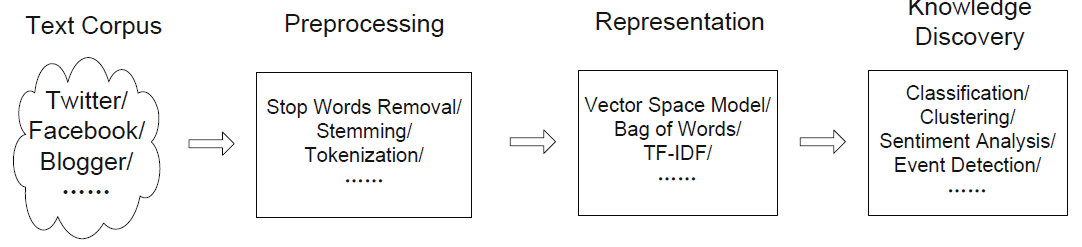
\includegraphics[height=0.25\linewidth, width=0.95\textwidth]{bilder/Abb2.png}
		\caption{Pipeline der Textklassifikation \citep{Kow19}  }\label{pipetk}
	\end{center}
\end{figure}
\subsection{Preprocessing}
Der rohe, unbehandelte Text wird beim \textit{Preprocessing} (deutsch: Vorbehandlung) in eine Form überführt, die eine nachfolgende Repräsentation der Daten durch Vektoren und ähnliche Methoden ermöglicht. Je nach gewünschter Anwendung sind hier verschiedene Vorverarbeitungsverfahren in Betracht zu ziehen.\\
Der Begriff Wortsegmentierung bzw. \textbf{Tokenisierung} bezeichnet die Zerteilung des Ausgangstexts in kleinere Einheiten, sogenannte \textit{Token} \citep{MannSch99}. In der Regel handelt es sich hierbei um einzelne Wörter, Zahlen und Satzzeichen. Als grundsätzliches Abgrenzungszeichen gelten in den meisten Sprachen die \textit{Whitespace}-Zeichen (Leerzeichen, Tab, Newline-Zeichen). Dies wird auch auf die zu analysierenden Tweets zutreffen, da diese fast ausschließlich in englischer Sprache verfasst sind.\\
\begin{figure}[htb]
	\begin{center}
		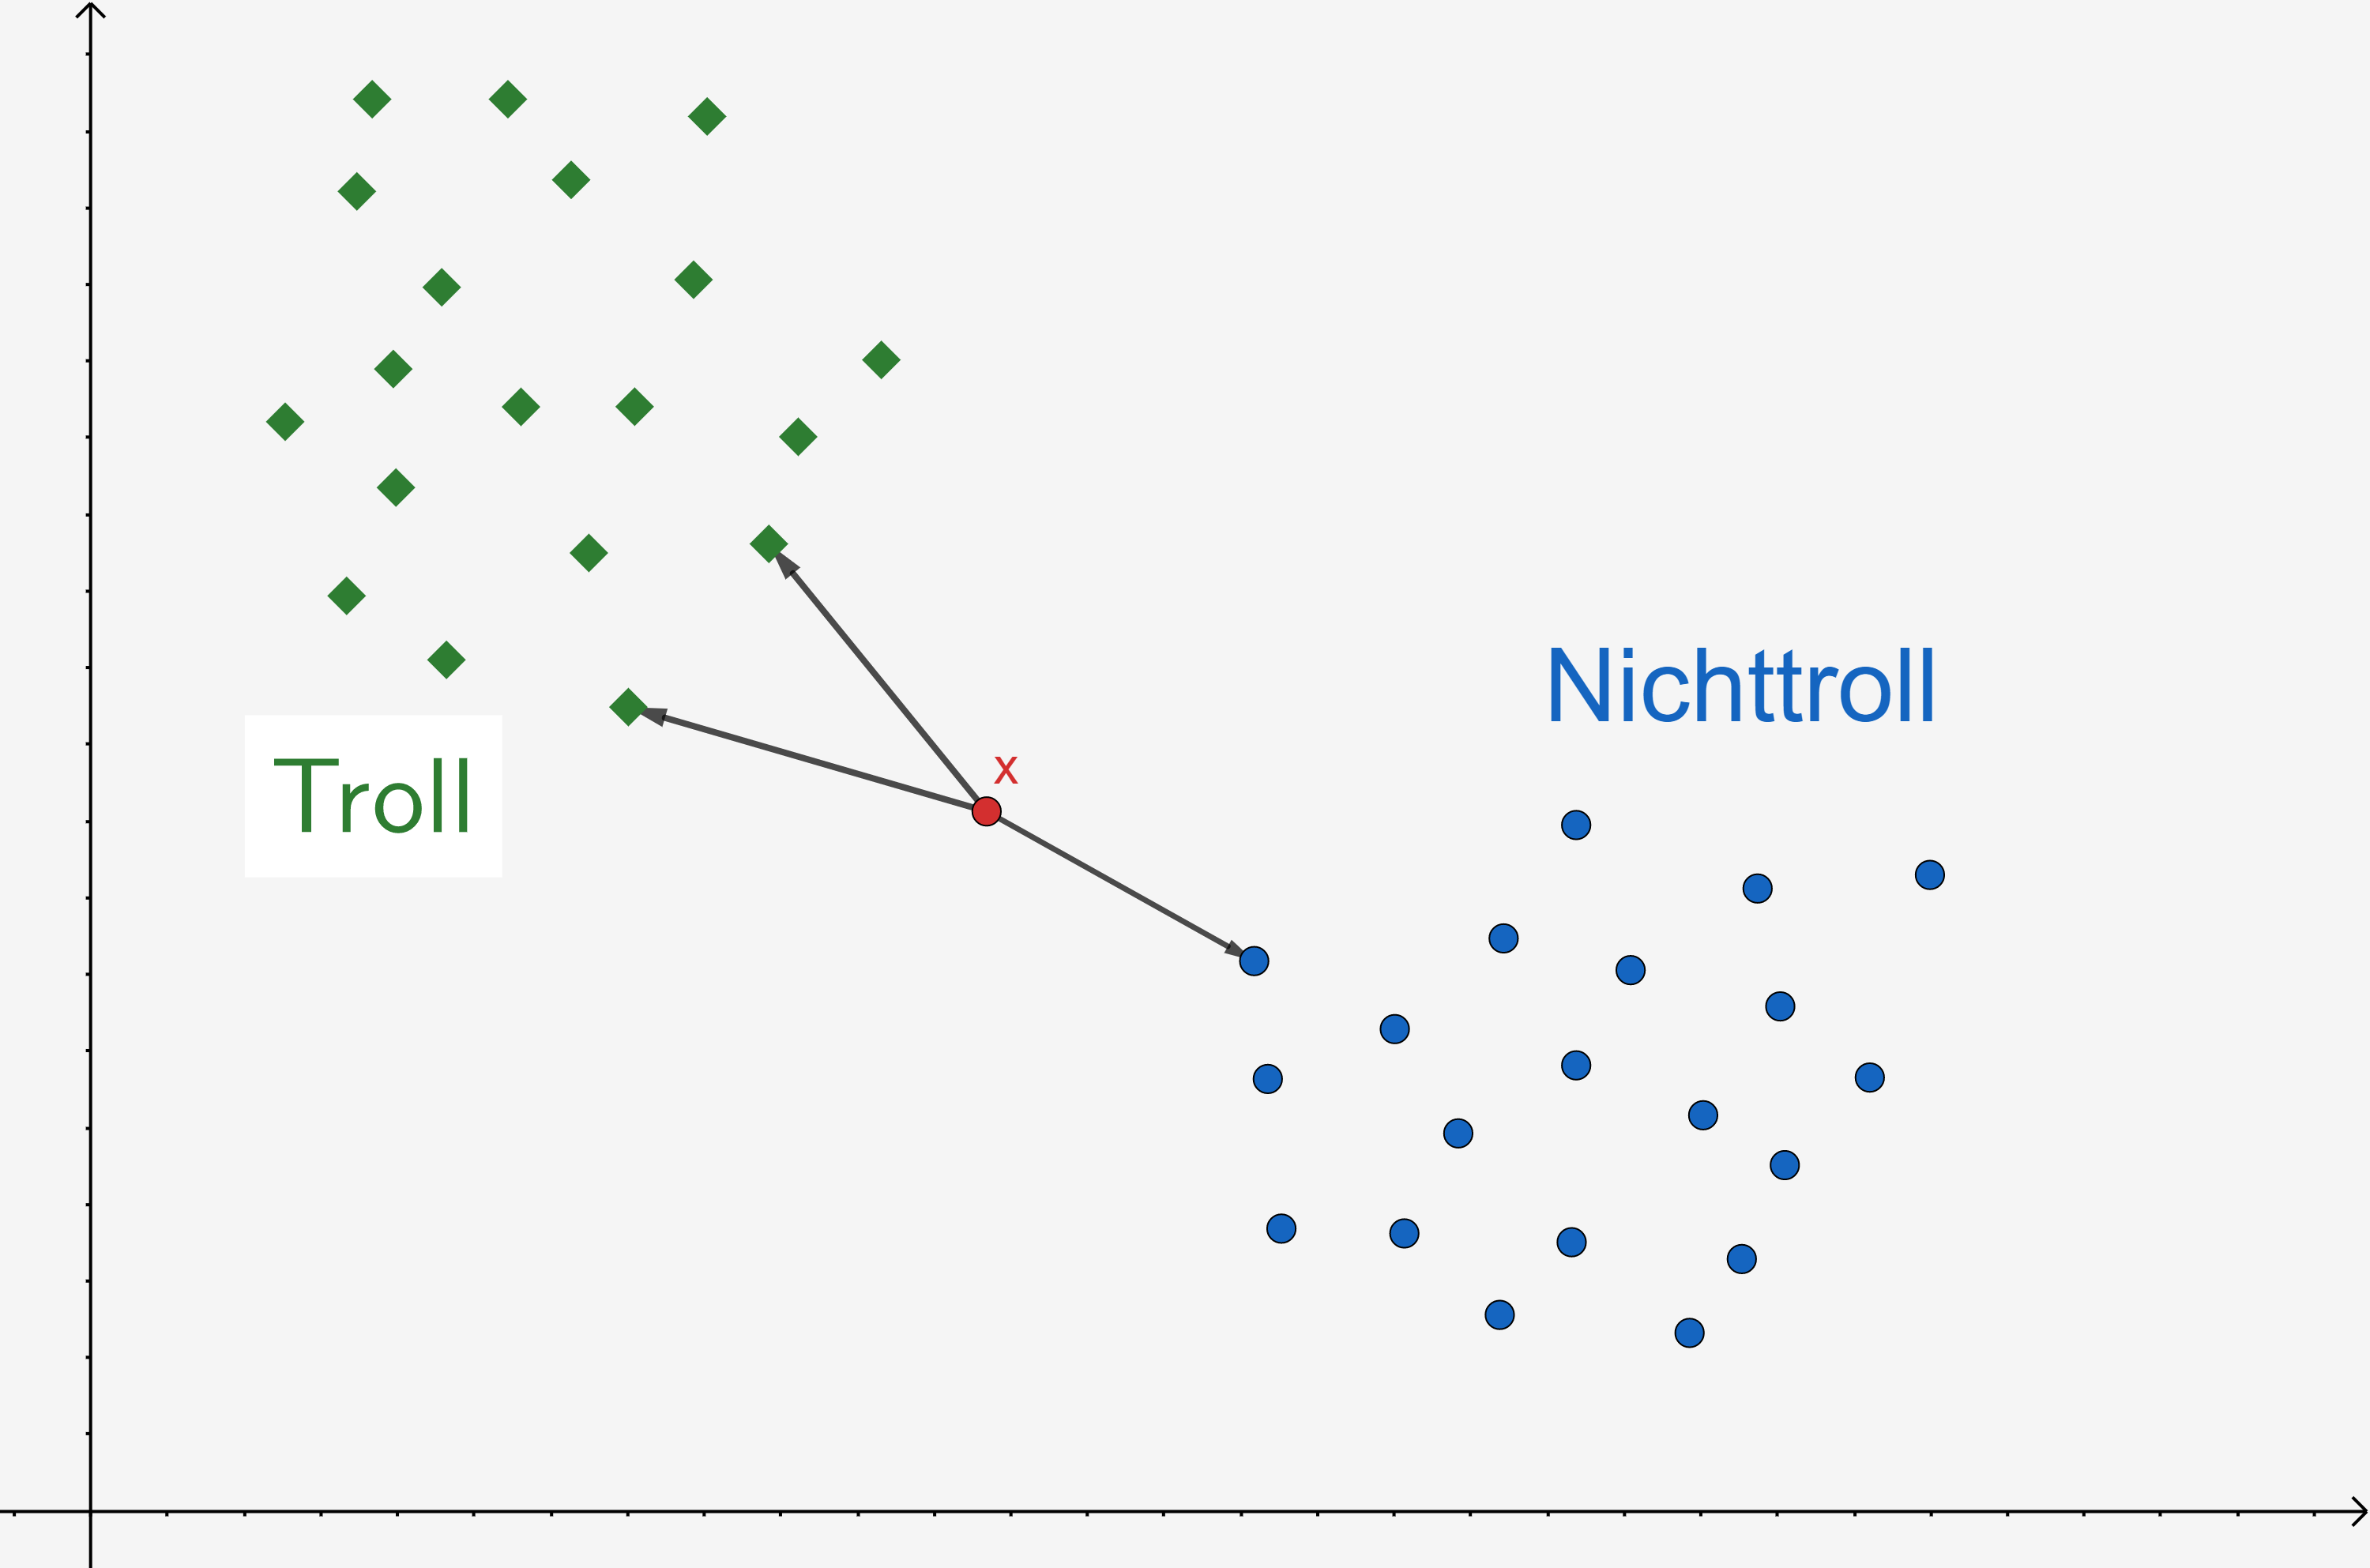
\includegraphics[width=\textwidth]{bilder/Abb3.png}
		\caption{Tokenisierung eines Beispielsatzes}\label{tokenization}
	\end{center}
\end{figure}\\
Eine weitere Methode der Vorverarbeitung ist das Entfernen von \textbf{Stoppwörtern}. Dies sind sehr häufig auftretende Wörter wie \glqq der\grqq, \glqq die\grqq, \glqq das\grqq, \glqq und\grqq{} oder \glqq von\grqq, welche vornehmlich eine grammatikalische Funktion und keinen Informationsgehalt haben. (vgl. ebd., S. 533)\\
Bei der \textbf{Lemmatisierung} \citep{Air06} werden mehrere Wörter unterschiedlicher Erscheinungsform, welche aber die gleiche Bedeutung haben, auf eine gemeinsame Grundform (genannt Lemma) zurückgeführt.  So lassen sich beispielsweise die deklinierten Substantive \glqq Wortes\grqq, \glqq Wörter\grqq, \glqq Wörtern\grqq auf \glqq Wort\grqq{} zurückführen, während die Grundform der konjugierten Verben \glqq schrieb\grqq, \glqq schreibe\grqq, \glqq schreibst\grqq{} und \glqq schreibt\grqq{} der Infinitiv \glqq schreiben\grqq ist. Ein verwandtes Konzept wird \textbf{Stemming} \citep{Air06} genannt. Der Unterschied zur Lemmatisierung besteht darin, dass das daraus resultierende Grundwort (hier: Stamm) kein natürlichsprachliches Wort sein muss, sondern in der Regel ein um Präfix und Suffix beschnittes Wort ist. Ein Beispiel hierfür ist die Reduzierung der Wörter \glqq gehen\grqq, \glqq umgehen\grqq und \glqq zugehen\grqq{} auf den Stamm \glqq geh-\grqq.\\
Für die Lemmatisierung eines Textes wird auch das \textbf{Part-of-Speech (POS) Tagging} \citep{Kuma15} benötigt. Hierbei wird einem Token seine Wortart (z.B. Nomen, Verb, Adjektiv) oder ein anderes Label wie \glqq Interpunktion\grqq{} zugewiesen. Werkzeuge, die dieses Verfahren anwenden, werden POS-\textit{Tagger} genannt.
\subsection{Feature Extraction}
Bevor eine Klassifikation vorgenommen werden kann, müssen die Merkmale aus den vorliegenden Texten gewonnen und mit mathematischen Methoden strukturiert bzw. modelliert werden. Hierbei fällt die Wahl zumeist auf Vektorisierung.\\
Die einfachste Vektorisierungstechnik ist die \textbf{Bag-of-Words} (BoW) \citep{Ramos13}. Hier wird ein Text durch einen Vektor mit den Begriffshäufigkeiten (auch: \textit{Term Frequencies} (\textbf{TF})) aller zuvor extrahierten Tokens des Textkorpus repräsentiert. Bei einem Beispielkorpus mit den beiden Texten \glqq my coffee is too hot\grqq{} und \glqq my tea is too cold\grqq{} und dem zuvor extrahierten Vokabular
\begin{flushleft}
	\hfil\{ "my", "coffee", "hot", "tea", "cold" \}
\end{flushleft}
ergibt sich die folgende Repräsentation:
\begin{flushleft}
	\hfil$v_1$ = [ 1, 1, 1, 0, 0 ]\\
	\hfil$v_2$ = [ 1, 0, 0, 1, 1 ]
\end{flushleft}
Eine Erweiterung dieser TF-Methode ist \textit{Term Frequency-Inverse Document Frequency} (\textbf{TF-IDF}) \citep{Ramos13}.  Hier wird die Vorkommenshäufigkeit anders gewichtet, um dem Aspekt gerecht zu werden, dass einige Begriffe überproportional oft vorkommen. Gleichung \ref{tfidf_weight} zeigt die Gewichtung 
\begin{equation}
	w(d,t) = TF(d,t) \cdot \log \left( \frac{N}{{DF}(t)} \right)
	\label{tfidf_weight}
\end{equation} 
wobei $N$ die Anzahl der Texte im Korpus und ${DF}(t)$ die Anzahl der Texte, welche den Begriff $t$ enthalten, ist.\\
Eine Möglichkeit, Wortkombinationen bzw. bestimmte Formulierungen als Merkmal zu berücksichtigen ist das \textbf{N-Gramm} \citep{Kow19}. Dies ist die Zusammenfassung von $N$ aufeinanderfolgenden Token in einem Text. Folglich handelt es sich bei den Elementen einer Bag of Words um 1-Gramme. Das nachfolgende Beispiel zeigt die Repräsentation des Textes \glqq Hier sehen Sie ein Beispiel.\grqq{} mit 2-Grammen:
\begin{flushleft}
	\hfil \{ \grqq Hier sehen \grqq, \grqq sehen Sie\grqq, \grqq Sie ein\grqq, \grqq ein Beispiel\grqq \}
\end{flushleft}
Alle vorausgegangenen Methoden der Merkmalsextraktion haben gemeinsam, dass sie keinen Aufschluss über Zusammenhänge der Wortbedeutungen (Semantik) geben. Dieses Problem versuchen die Techniken der \textbf{Worteinbettung} zu lösen. Ein prominentes Beispiel ist \textbf{Word2Vec} \citep{Mikolov13}. Die Grundidee ist hier, dass Begriffe, die eine ähnliche Bedeutung haben, in einem ähnlichen Kontext verwendet werden. Auf dieser Basis wird ein Vektor für jedes Wort im Vokabular durch ein neuronales Netz erzeugt. Die Entfernungen im daraus entstehenden Vektorraum geben dabei semantische Ähnlichkeiten wieder.
\subsection{Dimensionalitätsreduktion}
Bei sehr umfangreichen Datensätzen wie den mehr als 600.000 Tweets in dieser Arbeit werden in der Anwendung der zuvor beschriebenen Verfahren meist hochdimensionale Vektoren erzeugt. In der Folge werden viele Operationen bei späteren Algorithmen der Textklassifikation eine hohe Zeit- und Speicherkomplexität besitzen. Diesem Effekt versucht man im Voraus durch Dimensionalitätsreduktion entgegenzuwirken.\\
Ein erstes verwendetes Verfahren ist die Hauptkomponentenanalyse bzw. \textbf{Principal Component Analysis} (PCA) \citep{Jol02}. Mit diesem ist es möglich, in der Punktwolke der vorhandenen Vektoren all jene Vektor-Komponenten herauszufinden, die für die größte Varianz verantwortlich sind, also den größten Informationsgehalt haben. Der mathematische Mechanismus dahinter ist die Hauptachsentransformation: Es wird eine Ladungsmatrix aus den Eigenvektoren der Kovarianzmatrix gebildet, aus welcher der Anteil der Varianz jeder Komponente an der Gesamtvarianz ersichtlich ist. In der Folge können Komponenten, welche wenig Varianz beitragen, ohne nennenswerten Informationsverlust verworfen werden.\\
Eine andere Möglichkeit ist die \textbf{Nichtnegative Matrixfaktorisierung} (NMF) \citep{LeeSeung99}. Hier wird aus den $n$ Texten mit insgesamt $m$ Wörtern eine $m \times n$ Matrix gebildet, welche approximativ so faktorisiert wird, dass
\begin{center}
	$V \approx W H$
\end{center}
gilt, wobei W eine $m \times r$ Matrix und H eine $r \times n$ Matrix ist. Die $r$ Spalten von $W$ enthalten semantisch verwandte Wörter, welche zusammen einen Kontext bzw. ein Thema bilden. Voraussetzung für dieses Verfahren ist die Nichtnegativität von $V$.\pagebreak

%%%%%%%%%%%%%%%%%%%%%%%%%%%%%%%%%%%%%%%%%%%%%%%%%%%%%%%%%%%%%%%%%%%%%%%%
%%%% ENDE TEXTTEIL %%%%%%%%%%%%%%%%%%%%%%%%%%%%%%%%%%%%%%%%%%%%%%%%%%%%%
%%%%%%%%%%%%%%%%%%%%%%%%%%%%%%%%%%%%%%%%%%%%%%%%%%%%%%%%%%%%%%%%%%%%%%%%

\clearpage

% Entfernen Sie das Kommentar aus der nachfolgenden Zeile, falls Sie einen Anhang in der Arbeit verwenden wollen. Beachten Sie, dass Sie sich im Verlauf der Arbeit mit \ref{...} (z.B. \ref{anhang:zusatz1}) auf den Anhang beziehen.
%\newpage
\appendix
\section{Anhang}

\subsection*{Zusatzteil 1} \label{anhang:zusatz1}

Dies ist ein Anhang.

\clearpage



\ifthenelse{\boolean{\biber}}{ %with biber do
	\DeclareNameAlias{sortname}{first-last}
	\printbibliography[heading=bibintoc, title=\references]
}{ %without biber do
	\bibliography{references}
	\bibliographystyle{alphadin}
}
%\vspace*{\fill}


\clearpage

\listoffigures

\listoftables

%\pagebreak

%\printindex
\end{document}
